\documentclass[a4paper,10pt]{report}
\usepackage[utf8]{inputenc}
\usepackage{fullpage}
\usepackage{amsmath}
\usepackage{amsfonts}
\usepackage{tikz}
\usepackage{graphicx}
\usepackage{mdframed}
\usepackage{color}
\usepackage{listing}
\usepackage{wrapfig}
\usepackage[parfill]{parskip}
\usepackage{subcaption}
\usepackage{hyperref}
\usepackage[font={small}]{caption}
\usepackage{marvosym}
% Title Page
\title{Facet-based Imaging}
\author{Benjamin Hugo}
\date{April 2014}

\begin{document}
\maketitle
\chapter{Introduction to Radio Astronomy}
The focus of our work can best be summarized as accelerating the removal of artifacts introduced by creating widefield images from the measurements taken by radio telescopes. 
In this chapter a high level overview\footnote{It is important to stress that radio astronomy is a cross-section of many disciplines including astronomy, physics, 
electrical engineering and increasingly high performance and distributed computing. The following texts provide further insight to those coming from a computing background:
\begin{itemize}
 \item \textit{Antennas: Fundamentals, Design, Measurement (third, Blake \& Long)} serves as a good introductionary text on general [communications] radio antennae design from an electrical engineering perspective.
 \item \textit{Radiotelescopes (Christiansen \& H\"ogbom)} gives insight into the historic development of radiotelescopes from the 1930s through the 1960s, with a focus on telescope design and a good introduction
 to radio astronomy.
 \item \textit{A Scientist and Engineer's guide to Digital Signals Processing (Steven Smith)}\cite{smith1997scientist}. Available freely at \url{http://www.dspguide.com/}. An easy introduction to core digital 
 signals processing techniques, which cover sampling theory, introductory filter design and a good starter on the practical use of Fourier transforms.
 \item \textit{Synthesis Imaging In Radio Astronomy II (Taylor et al.)}. A very useful collection of lectures on synthesis imaging, covering the domain of radio astronomical imaging in its entirety.
 \item \textit{Interferometry and Synthesis in Radio Astronomy (second, Thompson, Moran \& Swenson)} covers the imaging pipeline in its entirety and serves as a valueble reference.
\end{itemize}
} of radio telescopes is given, including a discussion on what is being measured, how these telescopes work and ultimately how these 
measurements are related to images of the radio sky. We will then look at how to correct the distortions introduced when imaging over wider fields of view and finally on 
the technologies we will use to accelerate this widefield imaging process.
\section{Radio telescopes}
\subsection{Electromagnetic radiation}
Just as with visible light, radio waves are a form of electromagnetic radiation (consisting of waves with electrical and perpendicular magnetic components) which propagate through free space at the speed 
of light. We can conveniently measure these waves with telescopes of various form at either ground-level or from planetary orbit. This electromagnetic energy can be emitted by both thermal and non-thermal sources. 
The intensity of the radiation emited from thermal sources is determined by both the temperature of the source and the measured frequency. On the other hand a good example of non-thermal emission is the 
synchrotron emmision by relativistic electrons accelerated through magnetic fields. A significant portion of radio astronomy focusses on the non-thermal sources. These are generally very intense sources of 
electromagnetic radiation and are very far away. We can make the simplifying assumption here that source emits this radiation outward uniformly in all directions (they are \textit{isotropic} in other words) 
and that the distances over which they travel are far enough to consider them planar by the time they reach the observing telescope. 

One important factor to consider when measuring this incoming radiation with a telescope is the direction of propagation of each point on the incoming wavefront. If most of the energy of each wave is strongly 
directional the wave is said to be \textit{polarized}. For polarized emissions the path traced by a single point of the either the electrical or magnetic component will remain in a single plane (\textit{linear} polarization), 
will spiral at a fixed radius (\text{circular} polarization) or will be eliptical. Circular polarized electromagnetic radiation can be thought of as the combination of two perpendicular linearly polarized 
wavefronts of equal strength (if the two wavefronts are not equally strong the resultant polarization will be eliptical). We can draw on an application of this property from an everyday context: 
in the visible spectrum sunglasses will filter out all light except vertically polarized light, in order to reduce glare. A single-feed radio antenna will simularly measure a single directional component, and therefore only
useful in measuring strongly polarized sources. Such antennae are not useful for general observations, save for those of pulsars. In most contexts it is more useful to have two perpendular feeds (a dipole comes 
to mind) in order to fully describe the incoming wavefront (or at least the electric component thereof). When the energy measured by both feeds are roughly equal the emitting source is said to be \textit{unpolarized}.

In free space the propogation of these electromagnetic wavefronts is unempeded (obstructions or by any propagation medium) and the amplitude of these waves decay gradually with distance (proportional to 
the inverse square of the distance). However, this decay is not the only form of loss (or \textit{attenuation}) when these waves propagate through some medium other that a vacuum. In the atmosphere, 
depending on the wavelength of this radiation some particles such as oxygen and water vapour will absorb and scatter a significant portion of the incomming energy, and at very long wavelengths the charged 
ionosphere is effectively opaque. Due to these additional attenuation factors ground-based observation is effectively limited to the spectrum of visible light and the, vastly wider, radio band. Most of the 
in-between infrared spectrum is only observable at high altitudes and under dry conditions, see Figure~\ref{fig_radio_window}. 

\begin{figure}[ht]
 \begin{mdframed}
 \centering
 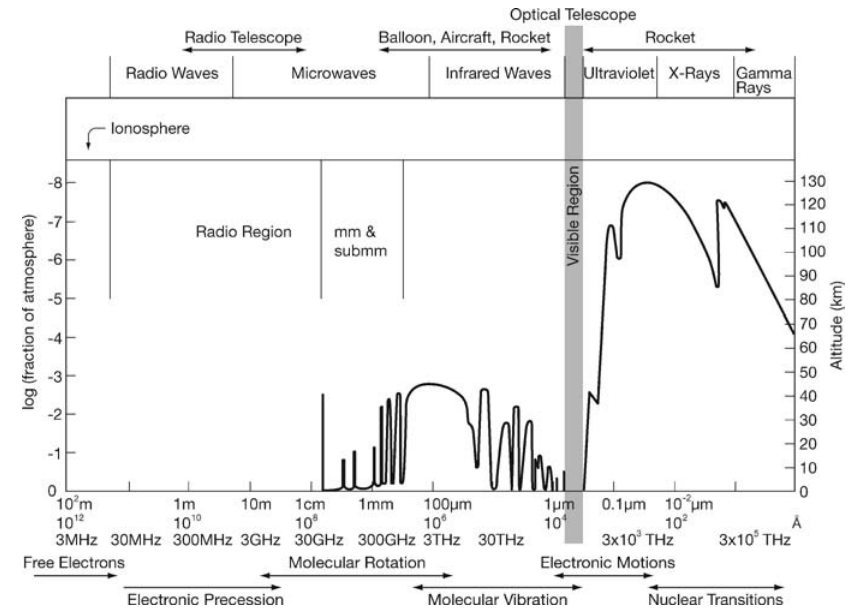
\includegraphics[width=0.6\textwidth]{images/radio_window.png}
 \caption[The radio window]{The radio window - Earth-based radio astronomy is bound to a range of wavelengths between $\lambda\approx 0.2mm$ and $\lambda\approx 20m$ by the molecular absorption bands of oxygen and water at the
 shorter wavelengths and the ionosphere at the long end. The figure shows at what altitude the incoming electromagnetic radiation is attenuated by a factor of 0.5 \cite{wilson2009tools}.}
 \label{fig_radio_window}
 \end{mdframed}
\end{figure}

In the early 1930s Karl Jansky's observation of radio electromagnetic radiation stemming from galactic sources far outside that of our home solar system have sparked interrest in observing this region of 
the spectrum. Since those early days we have seen significant increases in the sensitivity and size of these radio telescopes. We will start off explaining broadly how a single element telescope works, before 
moving onto the topic of apperture synthesis with array-based telescopes.
\subsection{Single element telescopes}
Maxwell's set of partial differential equations (1873) is one of the most elegant ways of explaining the relationship between electrical and magnetic fields, and how these can propagate at the speed of light 
though free space. In summary they state that a when current flows, a magnetic field is created in the surrounding space. When this magnetic field is varied an accompaning perpendicular electrical field is formed, varying
at the same frequency as the magnetic field, which in turn varies at the frequency at which the underlying current changes. Not only does this mean that antennae can generate electromagnetic fields and transmit signals (provided
sufficient input power), but in fact any transmitting antenna can be used as a receiver and vice versa (given it is capable of dealing with high voltages and is efficient enough for the particular application). Radio telescopes,
of course, take the form of receivers and, as with terrestial radio transmission and interference, the incoming extra-terrestial electromagnetic radiation will induce measurable current in the antenna (much more so at shorter 
wavelengths because of the opaqueness of the ionosphere at longer wavelengths).

Some of the most important measurements of a celestrial object includes the object's angular size, position (according to some celestrial coordinate system) and the \textit{flux} density over a 
frequency spectrum of the object. The flux density is measured as the power per square meter per unit frequency, falling on a surface, normal to the direction of the source. This flux 
density of sources is often a very small value and the Jansky (abbreviated Jy) serves as the unit of measure \cite{christiansenradiotelescopes,wilson2009tools}:

\begin{equation*}
 1 Jy := 10^{-26}Wm^{-2}Hz^{-1}
\end{equation*}

It is worth noting that, not only are radio telescopes used to observe spectra consisting of a wide band of frequencies, but for spectral line observations it is critical to observe narrow bands, with densely spaced channels. 
These spectral lines don't originate from large black-body structures, but focusses on the detection of certain molecules, such as neutral hydrogen (at $\lambda = 21 cm$) and
hydroxyl ($\lambda \approx 18 cm)$. These spectral lines are vital in measuring radial velocities through Doppler frequency shift \cite{christiansenradiotelescopes,taylor1999synthesis}.

It should be clear that since most sources are extremely faint, the telescopes needed to detect them will be some of the most sensitive instruments ever designed. Although we cannot
cover antenna theory extensively here, it is essential to briefly relate how the electromagnetic radiation covered earlier, is measured by instrumentation in general, as well as some of the constraints under which
these measurements are made.

The wave fronts from distant sources can be viewed as planar fronts if the source of the radiation is sufficiently far away. This is not necessarily true for sources within our own galaxy for example. Furthermore 
if the wavelength is much smaller than the scale of the phenomena the radiation can be viewed as rays. In radio astronomy these measures serve only as rough discriptions of the 
equations that govern wave propagation, as the wavelengths are significantly longer than in optical systems.  The total flux of a source is then obtained over the solid angle subtended by the 
source (see figure~\ref{fig_measuring_source_brightness}) as follows \cite{wilson2009tools}:

  \begin{equation}
    S_v := \int_{\Omega_s}{I_v(\theta,\phi)\cos{\theta}d\Omega}
  \end{equation}
  and the infinitesimal power intercepted by an infinitesimal surface is:
  \begin{equation}
    dP = I_v\cos{\theta}d\Omega\ d\sigma d\upsilon
  \end{equation}

  where:\\
  $dP = $ infinitesimal power (in watts)\\
  $d\sigma = $ infintesimal area of surface\\
  $d\upsilon = $ infintesimal bandwidth\\
  $\theta = $ angle between the direction to $d\Omega$ and normal to the surface\\
  $I_{v} =$ specific intensity in $Wm^{-2}Hz^{-1}sr^{-1}$ where r is the distance between the source and antenna.\\
  
\begin{figure}[ht]
\begin{mdframed}
 \centering
 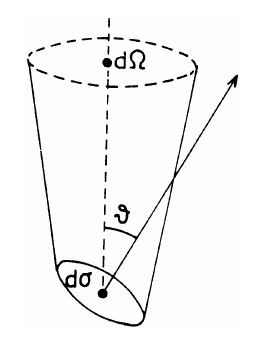
\includegraphics[width=0.2\textwidth]{images/measuring_source_brightness.png}
 \caption[Source brightness]{Flux density over a small area per unit frequency \cite{wilson2009tools}.}
 \label{fig_measuring_source_brightness}
\end{mdframed}
\end{figure}

For the sake of simplicity we will only consider a single simple parabollic reflector telescope for now to explain the general concepts of the primary beam and what impact it has on wide-field observations. Synthesis imaging \cite[ch. 3]{taylor1999synthesis} 
gives a more extensive overview of different antennae optics and mountings. Filled reflector antennas are normally used for $\lambda \geq 1m$, whereas unfilled ``wire'' antennae are frequently used at shorter wavelengths. We can describe
the operation of these parabollic reflectors using Huygen's principle \cite{christiansenradiotelescopes}: 
\begin{quote}
The energy at the focus of the telescope is the sum of the of the contributions from all parts of the incoming wave-front, taking into account the different path lengths and therefore different radio-frequency phases at the focus.
\end{quote}

The power available for a feed antenna placed at the focal point is proportional to the square intensity of the field of view and is known as the beam of the antenna and varies with the angle of incidence betweeen the the waves and the pointing of
direction of the antenna, see figure~\ref{diffraction_pattern_and_power_at_focus}. It should therefore be clear the telescope has a limited effective area of view. It turns out that the size of the aperture of the telescope plays a key role
in the resolving power of the telescope, which is limited by the diffraction patterns as seen in figure~\ref{diffraction_pattern_and_power_at_focus}. Any object larger than the primary beam of the antennae will be aliased to a certain
extent by the sidelobes shown in figure~\ref{diffraction_pattern_and_power_at_focus}, although the general structure may still be the same:
\begin{equation*}
 \text{resolving power} \propto \frac{\lambda}{D}
\end{equation*}
\begin{figure}[ht]
 \begin{mdframed}
  \centering
  \begin{subfigure}[b]{0.3\textwidth}
   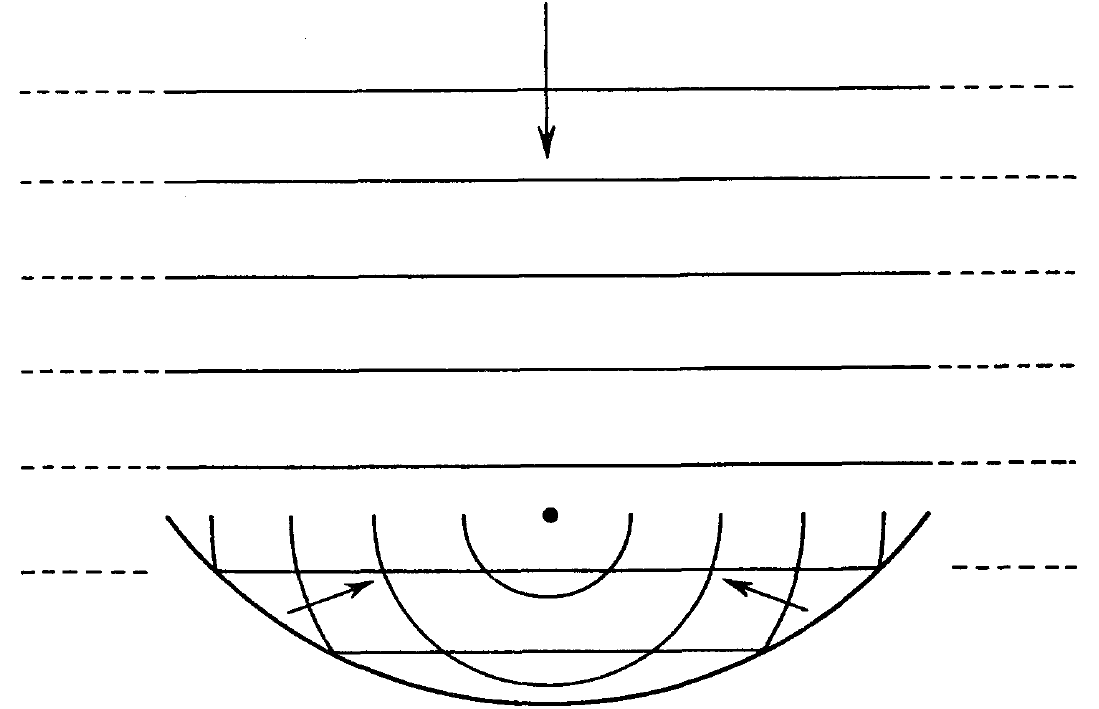
\includegraphics[width=\textwidth]{images/diffraction_pattern.png}
   \caption{}
  \end{subfigure}
  \begin{subfigure}[b]{0.3\textwidth}
   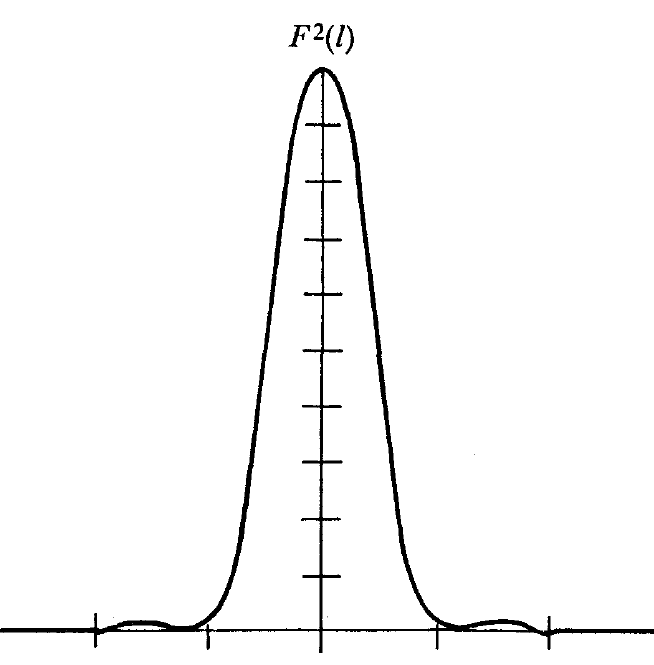
\includegraphics[width=\textwidth]{images/field_strength_in_the_focal_plane.png}
   \caption{}
  \end{subfigure}
  \begin{subfigure}[b]{0.3\textwidth}
   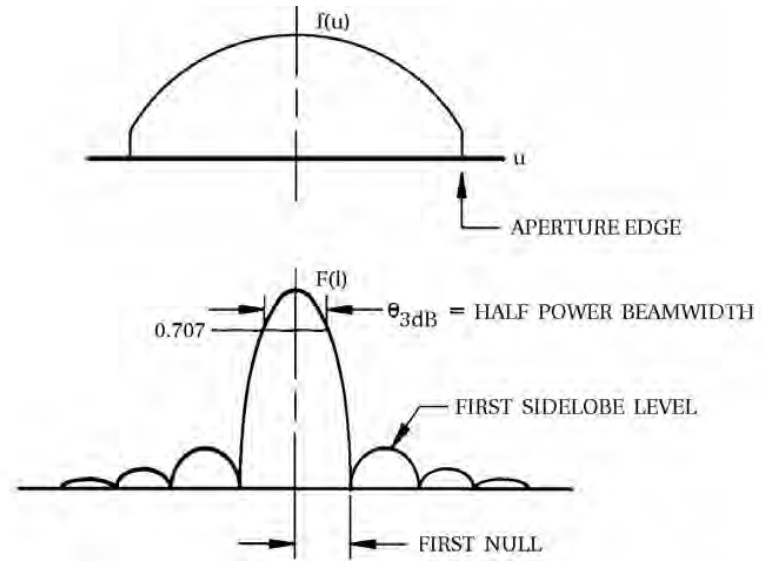
\includegraphics[width=\textwidth]{images/radiation_pattern.png}
   \caption{}
  \end{subfigure}
  \caption[Collection of electromagnetic wave energy and responce]{In (a) we illustrate the defraction pattern of a parabollic aperture and how the total energy is collected at the focal point \cite{christiansenradiotelescopes}. This is similar to the diffraction pattern of
  visible light caused by passing through a single narrow slit. In (b) the power at the antenna terminals is significantly higher for small angles from the antenna pointing direction \cite{christiansenradiotelescopes}. Lastly in (c) we give a 1 dimensional illustration of 
  the effects of apperture form and diameter on the antenna's effective resolving capability. If objects larger than the center beam is observed the objects will be effectively aliased by the ``sidelobes'' off both ends of the ``primary'' beam. The response is the \textit{fourier transform} 
  of the shape of the aperture. It should now be clear that the effective collection area, $A(l,m)$ approaches the geometric area of the apperture in the direction of maximum response \cite{taylor1999synthesis}.}
  \label{diffraction_pattern_and_power_at_focus}
 \end{mdframed}
\end{figure}

Another key observation to take into consideration are the effects of polarization in electomagnetic wavefronts. All electromagnetic radiation can be characterised by a field vector parallel to to the wavefront. This wavefront is said to
be either elliptically polarized if the field vector traces out an ellipse of constant orientation and eccentricity (linear and circular polirization are special cases of this). On the other hand it may be randomly polarized (or ``unpolarized'') if the field 
vector changes randomly. To capture the total energy of of the electromagnetic field any antenna should have two independent feeds to resolve any radio wave, where the second feed must be placed at right angles to the first. The first and second feeds will carry, 
on average equal amounts of power. The total flux density is therefore the sum of both polarized feeds \cite{christiansenradiotelescopes}.

Up to this point we've assumed that the energy measured at the focus point of the telescope is attributed to a single point source. In reality many sources contribute to the specific intensity integral over the solid angle $d\Omega$. These point sources
are generally accepted to be completely uncorrelated, and therefore the mean squared voltage at each of the antenna feeds is a linear combination from each of these sources (weighted by the effective area function $A(l,m)$) \cite{christiansenradiotelescopes}. In general this requires instrument 
calibration to be done over all the bright sources in the beam-limited field of view. More on calibration techniques later on.

\section{Interferometric telescopes}
As pointed out in the previous section the angular resolution is constrained to the diameter of the telescope. Unfortunately there are material constraints to the size of an apperture ($\sim 300m$ as pointed out in \cite{wilson2009tools}). The Arecibo Observatory, Puerto Rico is the extreme case 
of this, see fig~\ref{fig_arecibo}. Luckily the same resolving power may also be obtained by \textit{coherently} combining the feeds from two reflectors, seperated by a straight-line distance, $B$:
\begin{equation*}
 \text{resolving power} \propto \frac{\lambda}{B} \text{ if } D\ll B
\end{equation*}
\begin{figure}[ht]
 \begin{mdframed}
 \centering
 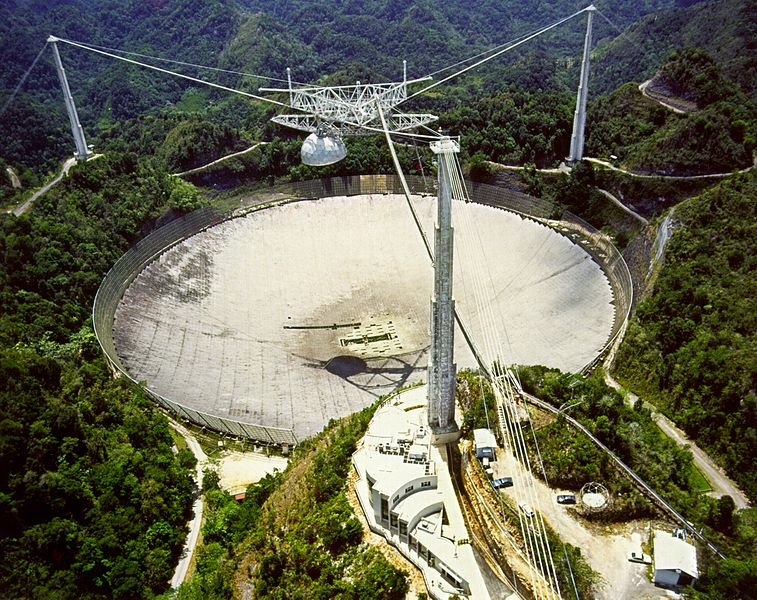
\includegraphics[width=0.7\textwidth]{images/arecibo.jpg}
 \caption[Arecibo Observatory]{At a wopping 305m diameter, the telescope at the Arecibo Observatory is the largest single-apperature telescope in the world. Image courtesy of the National Oceanic and Atmospheric Administration (public domain).}
  \label{fig_arecibo}
 \end{mdframed}
\end{figure}

This combination process synthesizes a larger aperture (in general this aperture is unfilled \cite{christiansenradiotelescopes}), with the first practical demonstration made by Ryle and his associates. The feeds from two antennae are joined by a 
correlator which, can be thought of, as taking short-time averages to measure the difference in phase between two signals. When the antennae are spaced $B$ units appart the electromagnetic wavefront will reach one telescope before reaching the 
other (figure~\ref{fig_cosine_correlator}). This delay, $\tau=\frac{\vec{b}\cdot\hat{s}}{c}$ is usually compensated for by the correlator in order to achieve a coherent correlation (as mentioned previously). For short intervals the correlator 
response (for a planar wavefront) over all the sources in the effective collection area, projected onto a \textit{baseline} $\vec{b}$, is given as (refer to figure~\ref{fig_cosine_correlator}) \cite{taylor1999synthesis}:
\begin{equation}
\label{eqn_cosine_correlation}
r=\Delta\upsilon \int_{\vec{s}}{A(\vec{s})I(\vec{s})\cos{\frac{2\pi\vec{b}\cdot(\vec{s}-\vec{s_0})}{\lambda}}d\Omega}
\end{equation}

\begin{figure}[ht]
 \begin{mdframed}
 \centering
 \begin{subfigure}[b]{0.3\textwidth}
 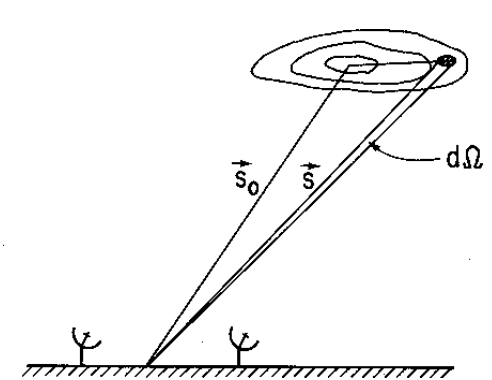
\includegraphics[width=\textwidth]{images/phase_center.png}
 \caption{}
 \end{subfigure}
 \begin{subfigure}[b]{0.4\textwidth}
 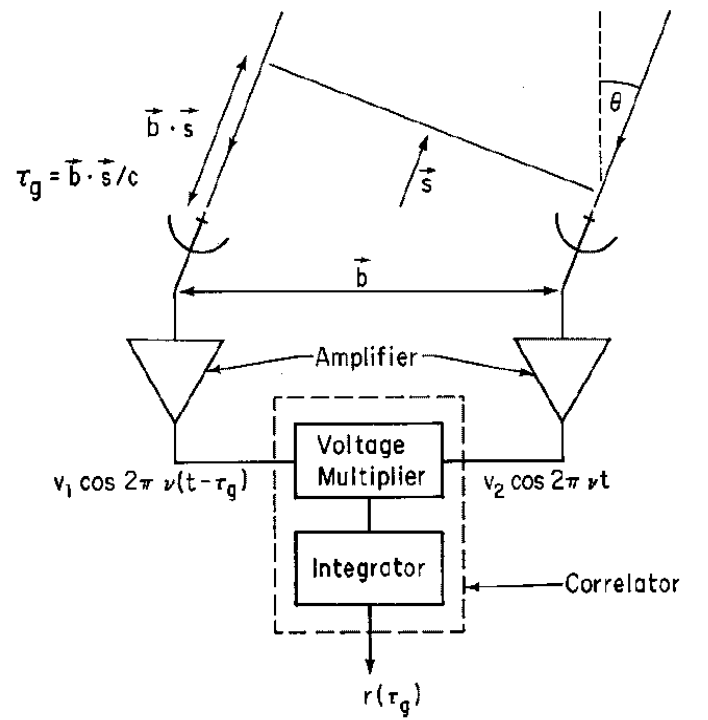
\includegraphics[width=\textwidth]{images/cosine_correlator.png}
 \caption{}
 \end{subfigure}
 \begin{subfigure}[b]{0.2\textwidth}
 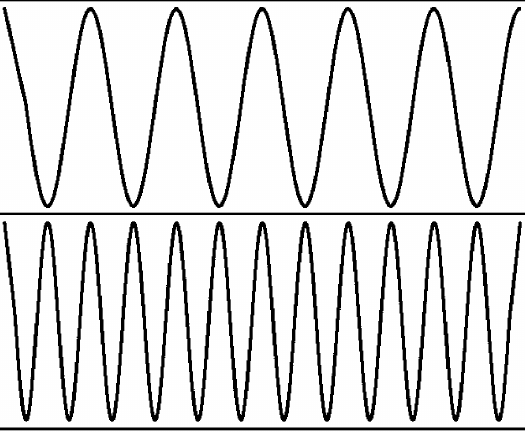
\includegraphics[width=\textwidth]{images/fringe.png}
 \caption{}
 \end{subfigure}
 \caption[Cosine correlator]{(a) Position vectors used in the interferometer response. $\vec{s_0}$ is the \textit{phase tracking center} where $\tau:=0$ \cite{taylor1999synthesis} (b) Simplified diagram of a two-element correlator, combining the output of two elements spaced $B=||\vec{b}||$ appart. The integrator takes the \textit{cross correlation} of the signal 
 from the second telescope and a time-delayed signal from the first telescope over a small period of time \cite{taylor1999synthesis}. (c) The power produced through cross correlation, differs from that of a single element telescope as shown in figure~\ref{diffraction_pattern_and_power_at_focus} and has a response for greater angles than a small single reflector telescope. If $B$ is doubled, 
 the fringe width is halved and the the correlator response for larger angles improves. This process is analoguous to the diffraction of visible light in Young's double-slit experiment. \cite{wilson2009tools}.}
  \label{fig_cosine_correlator}
 \end{mdframed}
\end{figure}
It is easy to see that this correlator ``fringe'' pattern has a major drawback: the correlator is insensitive for $\frac{2\pi\vec{b}\cdot(\vec{s}-\vec{s_0})}{\lambda} = \frac{\pi}{2} \pm n\pi$. To fix this problem correlators typically
take the form of \textit{complex correlators} where a second correlation is made by introducing a phase delay of $\frac{\pi}{2}$ in the feeds of the antennae. The second correlator is effectively a \textit{sine correlator}. We can
now replace the cosine term in equation~\ref{eqn_cosine_correlation} by $e^{-2\pi\vec{b}\cdot(\vec{s}-\vec{s_0})/\lambda}$ through the Euler relation between the complex exponential and the polar form of a complex coordinate \cite{taylor1999synthesis}.

The next issue are the effects of limited \textit{bandwidth}, $\Delta\upsilon$, in correlators. Since it is computationally infeasible to sample an infinite spectrum of frequencies, only a select number of channels are sampled. This
band is normally shifted down to \textit{baseband} ($\upsilon=0$) and filtered appropriately with a lowpass filter to reduce aliasing, refer to figure~\ref{fig_bandwidth}. The baseline is normally measured in wavelengths and therefore depends on the
center frequency through the well-known relation $\upsilon=\frac{c}{\lambda}$. Unfortunately this has a negative impact on the fringe pattern of the correlator; for a rectangular frequency band the fringe is modulated by a sinc-function. This has
the effect of tapering the fringe which again reduces the effective area of the interferometric telescope. The obvious solution is to observe only narrow spectra. The fringe additionally depends on the delay term and oscilates in time. Normally this is not a problem. However, with exceedingly long baselines such as those in \textit{Very Long Baseline Interferometry}, where the baselines may span continents (see Middelberg et al. \cite{middelberg2008high} for a detailed overview), the local oscilator term is usually varied 
by a delay tracking computer, which essentially stops any fringe oscilation (known as \textit{fringe stopping}) \cite{taylor1999synthesis}.
\begin{figure}
 \begin{mdframed}
 \centering
 \begin{subfigure}[b]{0.3\textwidth}
 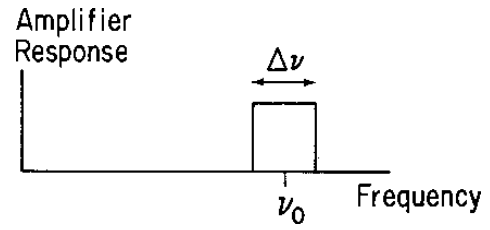
\includegraphics[width=\textwidth]{images/rectangular_band.png}
 \caption{}
 \end{subfigure}
 \begin{subfigure}[b]{0.5\textwidth}
 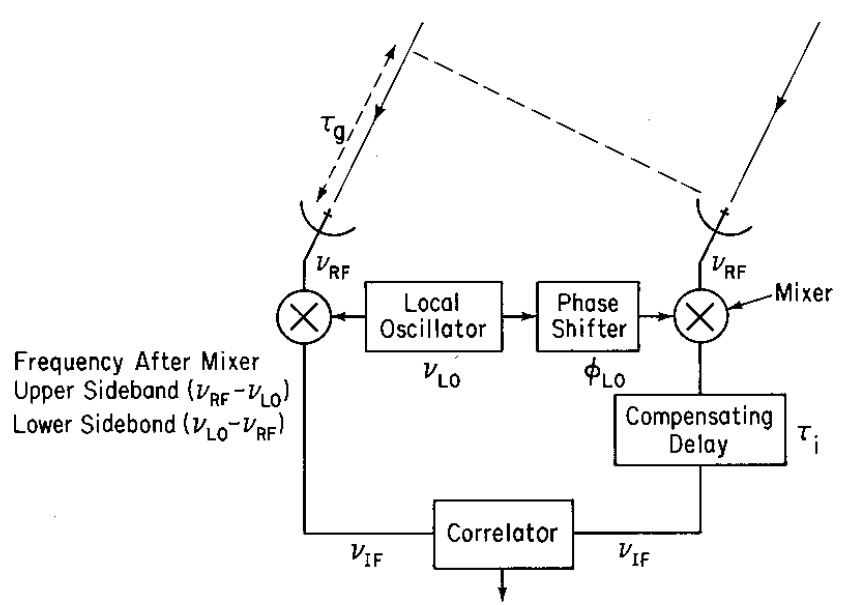
\includegraphics[width=\textwidth]{images/mixing.png}
 \caption{}
 \end{subfigure}
 \caption[Sampling a limited bandwidth]{(a) illustrates the idealized rectangular responce of the correlator. Due to inevitable filter rolloff this is obviously unatainable \cite{taylor1999synthesis}. (b) For practical
 reasons the signal is shifted to baseband before filtering out higher frequencies. This is achieved by multiplying the signal with a tone produced by a local oscilator (mixing) this shifts the 
 frequency response of the correlator by $\pm\upsilon_{lo}$ \cite{taylor1999synthesis}} 
  \label{fig_bandwidth}
 \end{mdframed}
\end{figure}

Up to this point we conveniently only discussed correlator output for a single feed of each antenna in a two element interferometer. The correlator \textit{may} additionally cross-correlate the two polarization feeds to 
form the following matrix of correlation components between the antennae p \& q (where * indicates the complex conjugate). In instances where all of these components are available may the Stokes parameters (I, V, U and Q) be computed. 
The equation governing the correlator power response remain the same for the four different polarizations.  \cite{taylor1999synthesis}.
\begin{equation}
    \left[\begin{array}{c c}
     <e_{X_p}e_{X_q}^*> & <e_{X_p}e_{Y_q}^*> \\
     <e_{Y_p}e_{X_q}^*> & <e_{Y_p}e_{Y_q}^*> \\
    \end{array}\right] \approx 
    \left[\begin{array}{c c}
     I + V & Q + iU \\
     Q - iU & I - V \\
    \end{array}\right] = B
\end{equation}
Each of the parameters Q, U and V are linearly independent and discribe a position on the Poincar\'e Sphere (figure \ref{fig_poincare}). Their coordinates on the sphere are given by
\begin{equation}
  \begin{split}
    Q &= I\cos{2\chi}\cos{2\psi}\\
    U &= I\cos{2\chi}\sin{2\psi}\\
    V &= I\sin{2\chi}\\
  \end{split}
\end{equation}

\begin{figure}
 \begin{mdframed}
 \centering
 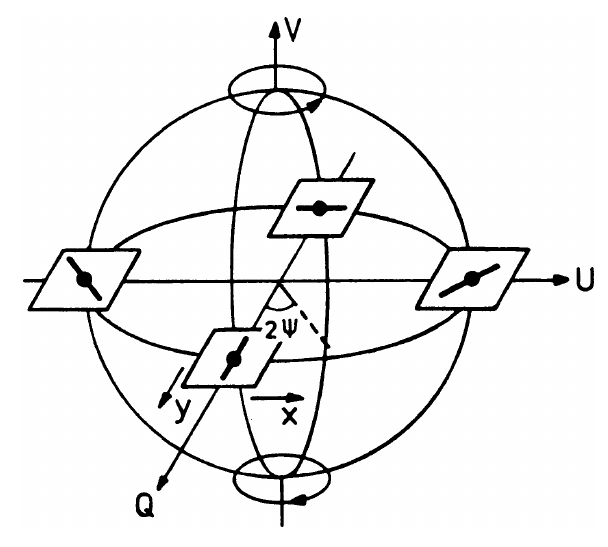
\includegraphics[width=0.45\textwidth]{images/poincare_sphere.png}
 \caption[The Poincar\'e Sphere]{The Poincar\'e Sphere gives a visualization for the different polarizations an electromagnetic field. The angles $2\psi$ and
 $2\chi$ are the angles in a polar coordinate system, with each point on the sphere corresponding to a unique polarization. At $2\chi=0$ (the equator) the polarizations 
 are either linear (Q) and orthagonal (U). The northern latitudes ($2\chi > 0$) contain right-handed circular polarization, while the southern hemisphere 
 contains the left-handed circular polarizations. $I$ is not linearly independent and describes the total Poynting flux of the electromagnetic wave; $I = E_1^2 + E_2^2$ \cite{wilson2009tools}}
  \label{fig_poincare}
 \end{mdframed}
\end{figure}

It is worthwhile to note that the correlation, delay and phase compensations can also be done in the fourier domain, and in the case of delay compensation this approach makes fractional delay compensation feasible (see Taylor et al. \cite{taylor1999synthesis}). These correlators are effectively 
known as \textit{FX} correlators. If these power spectra are of high time resolution it is possible to perform surveys focussed on transient detection. Modern arrays such as LOFAR, KAT-7 and MeerKAT (currently under construction) have the capability to perform these searches through
special \textit{beamforming} modes which may be run concurrently with imaging modes. See Stappers et al. \cite{stappers2011observing} for details on pulsar observation with LOFAR. In this thesis, however, we will focus solely on the imaging pipeline which is discussed in the next section.

\section{The fundamentals of array-based imaging}
\subsection{The all-sky Radio Interferometric Measurement Equation}
In the previous section the response, $r$, of a complex correlator was described. The \textit{visibility} is an unnormalized measure of the coherence of an electric field, and is very closely related to the correlator response to the planar wave fronts emitted
by a source. The magnitude of this coherence has dimensions of flux density as described earlier. The Radio Interferometric Measurement Equation relates between these visibilities and the projection of the source onto the celestial sphere. This projection and measurement
process is illustracted in figure~\ref{fig_uvw_lmn}. Without loss of generality when extended to the different polarization terms, the relation between the measured visibilities and the image can be defined as:
\begin{equation}
 \label{eqn_visibility}
 \begin{split}
  V(u,v,w) &:= \int_{\vec{s}}{A(\vec{s})I(\vec{s})\cos{\frac{2\pi\vec{b}\cdot(\vec{s}-\vec{s_0})}{\lambda}}d\Omega}\\
	   &= \int_{-\infty}^\infty{\int_{-\infty}^\infty{A(l,m)I(l,m)e^{-2\pi i[ul+vm+w(n-1)]} \frac{dldm}{\sqrt{1-l^2-m^2}}}}\\
	   &= \int_{-\infty}^\infty{\int_{-\infty}^\infty{A(l,m)I(l,m)e^{-2\pi i[ul+vm+w(\sqrt{1-l^2-m^2}-1)]} \frac{dldm}{\sqrt{1-l^2-m^2}}}}
 \end{split}
\end{equation}

\begin{figure}[h]
 \begin{mdframed}
 \centering
 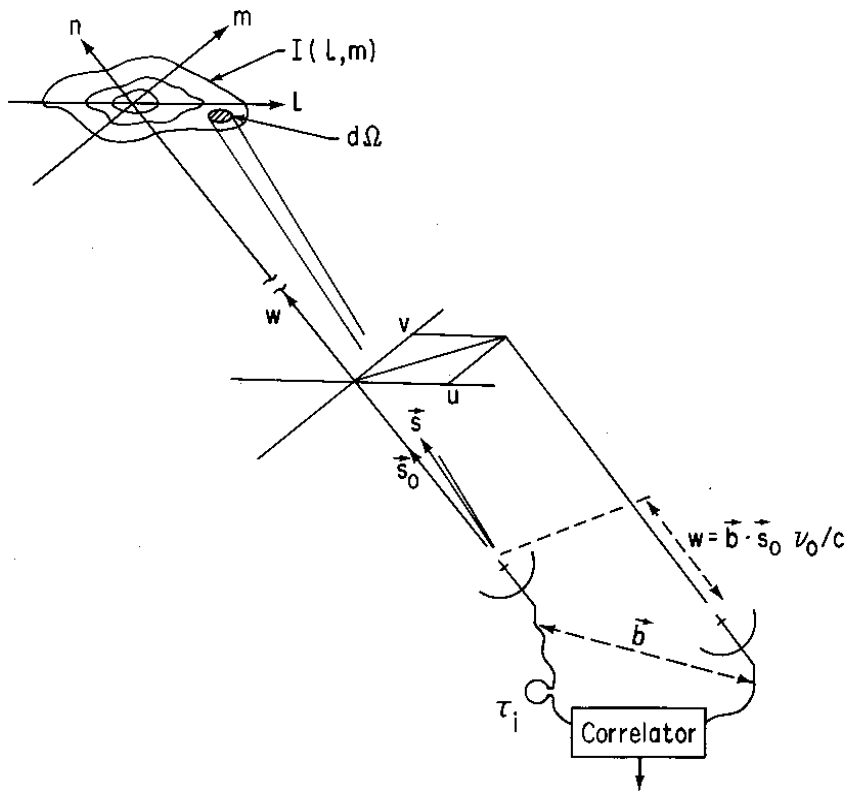
\includegraphics[width=0.5\textwidth]{images/lmn_uvw.png}
 \caption[The relation between image space and visibilities]{The relation between the measured spatial coherence function and the source on the unit ``celestial'' sphere, emitting planar waves of radiation \cite{taylor1999synthesis}.}
  \label{fig_uvw_lmn}
 \end{mdframed}
\end{figure}

Typically some reference point is used to specify the relative positions of the Antennae. The baseline is then given by the following relation, where $H_0$ and $\delta_0$ is the respective hour angle and declanation of the 
phase reference center and $\lambda$ is he wavelength corresponding to the center frequency of the receiver as mentioned previously. Refer to figure~\ref{fig_celestrial_coords} for a visual reference of the celestrial 
sphere, and the equatorial and alt-azimuth coordinate system.
\begin{equation}
 \left[\begin{array}{c}
     u\\
     v \\
     w \\
    \end{array}\right] = \frac{1}{\lambda}
 \left[\begin{array}{c c c}
     \sin{H_0} 			& \cos{H_0}			& 0 \\
     -\sin{\delta_0}\cos{H_0} 	& \sin{\delta_0}\sin{H_0}	& \cos{\delta_0}\\
     \cos{\delta_0}\cos{H_0} 	& -\cos{\delta_0}\sin{H_0}	& \sin{\delta_0}\\
    \end{array}\right]   
 \left[\begin{array}{c}
     L_X \\
     L_Y \\
     L_Z \\
    \end{array}\right]
\end{equation}

\begin{figure}[h]
 \begin{mdframed}
 \centering
 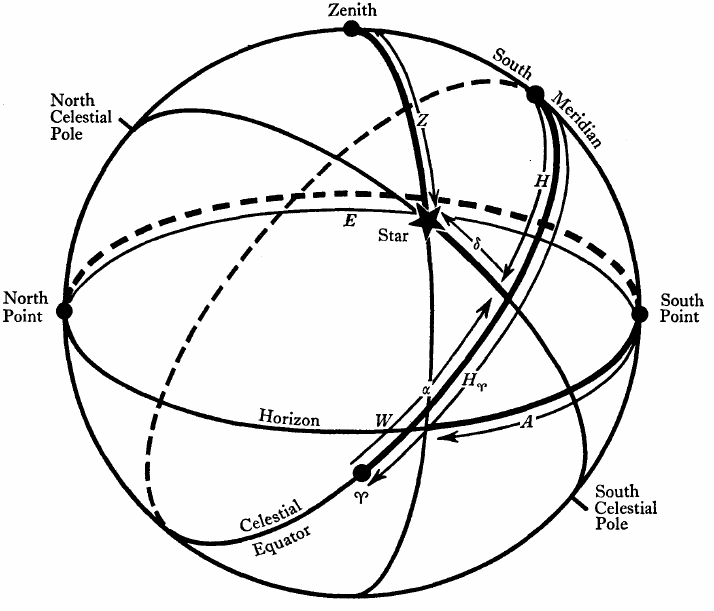
\includegraphics[width=0.75\textwidth]{images/equatorial_coords.png}
 \caption[Equatorial and alt-azimuth coordinate system]{The angular coordinates of a point in space is usually measured in terms of declination ($\delta$) and either right-ascension ($\alpha$ or R.A.) or the hour angle ($H$) from the place
 where observations are taken. The first point of Aries (\Aries) is the position of the Sun at the March Equinox. The celestrial equator is simply Earth's equator projected onto the celestial sphere. There is normally a slow precession in the Earth's
 axis and this has to be corrected for, based on some reference point in time (an epoch). The last epoch at the time of writing was at noon January 1, 2000. See Radiotelescopes \cite[Appendix 4]{christiansenradiotelescopes} for more information.}
  \label{fig_celestrial_coords}
 \end{mdframed}
\end{figure}

When the field of view being observed is sufficiently small, $n$ is close to unity and the term $w(n-1) = 0$. Similarly, if the all the antenna are at equal height (\textit{co-planar}) $w=0$ and the term disappears as well. Under 
these circumstances equation~\ref{eqn_visibility} is the two dimensional fourier transform of the image. In reality the image is not only affected by the effective area of the comprising elements in the interferometer, but is 
subject to incomplete sampling, direction-independent antenna gains, as well as directional effects, such as ionospheric and tropospheric conditions. 

Equation~\ref{eqn_visibility} may thus be rewritten to take multiple polarizations, the gains and directional effects into account through a \textit{Jones} matricies formulation presented by Smirnov in a series of papers on the 
formulation and its implications for calibration \cite{2011A&A...527A.106S,2011A&A...527A.107S,2011A&A...527A.108S}. Here the B term is the Stokes parameter matrix as we defined in the previous section (B may represent either
linear or circular polarizations, with the necessary coordinate system transformations added):

\begin{equation}
\label{eqn_RIME}
\begin{split}
    V_{pq} &= G_p(t,\upsilon)\left(\int_{-\infty}^{\infty}\int_{-\infty}^{\infty}D_p(l,m,t,\upsilon)BK_{pq}D_q(l,m,t,\upsilon)^H\frac{dldm}{\sqrt{1-l^2-m^2}}\right)G_q(t,\upsilon)^H\\
	  &\text{where }K = e^{-2\pi i(u_{pq}l+v_{pq}m+w_{pq}(n-1))}
    \left[\begin{array}{c c}
     1 & 0 \\
     0 & 1 \\
    \end{array}\right]\\
	 &\text{and the G terms are the direction-independent effects,}\\
	 &\text{while the D terms are dependent on the direction of the source in l,m space}\\
 	 &J^H:=\bar J^T \text{ indicates the Hermitian transpose (or the transpose of complex conjugate matrix of all the J indicies)}\\ 
\end{split}
\end{equation}

The fundamental assumption here is that all effects on the measured intensities are linear and can therefore be written as two-dimensional matricies. Each antenna will additionally have its own set of these effects. 
They include corrections for Faraday rotation, ionospheric effects, tropospheric effects and pointing error due to weather (wind and heat). These corrections only account for amplitude scaling and phase shifts and can be 
combined in a layered approach by multiplying several of these Jones terms together (note that the terms may not necessarily commute, so the order of multiplication is important). The different effect effects will be described 
later when calibration is discussed.

\subsection{Array-based observation}
Each observation will typically extend over a prolonged period of time (over many hours for instance) and collect a large number of visibilities, typically over a large number of channels. As the earth rotates each baseline sweeps out
eliptical paths in u,v space, sampling the coherence function at regular intervals. As the number of antennae in the array is increased the number of measured visibilities grow quadratically, since the number of possible baselines between 
antennae is given as $\frac{n(n-1)}{2}+n$. Adding a small number of antennae to the array can therefore effectively improve the uv coverage. By adding more visibilities in fourier space the quality of the synthesized 
image is improved, because the effects of the limited sampling can be more effectively removed from the produced image as is explained in the section on convolutional gridding.

The uniform and wide coverage of the entire u,v space (the size of which is determined by the required angular resolution), can normally be attained using only east-west baselines, except at very low declanations (less than about $30^o$) at the horizon. At low declanations baselines 
with a component sufficiently parallel to the Earths axis (non East-West) are needed. Such a two dimensional array have baseline components which don't remain co-planar over long observations and require the l and m components being small enough to 
ensure $(\sqrt{1 - l^2 - m^2} - 1)w \approx 0$. See figure~\ref{fig_VLBA_uv} for an illustration of the uv-coverage attained by the VLBA array. The spacing in such an East-West array is of high importance
in ensuring the uniform sampling of the u,v space. Spacing the antennas uniformly for instance will result in many redundant coverages by the shorter baselines. Other designs include movable
antennae provide greater flexibility and can cover more baselines. For two dimensional arrays reducing redundancy becomes even more challenging as eluded to in Synthesis Imaging II \cite[Lecture 2]{taylor1999synthesis}.

\begin{figure}[h]
 \begin{mdframed}
 \centering
 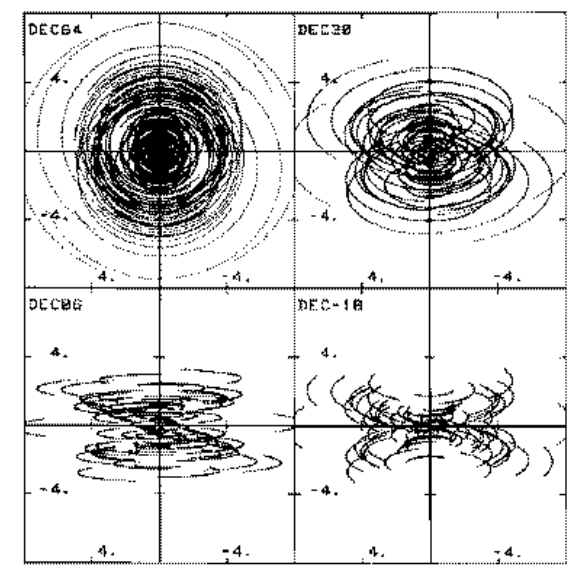
\includegraphics[width=0.5\textwidth]{images/eliptical_sampling.png}
 \caption[VLBA uv-coverage]{The sampling patterns of the ten antennae of the VLBA at 4 different declanations. The best coverage is attained at greater declanations}
  \label{fig_VLBA_uv}
 \end{mdframed}
\end{figure}

\subsection{Telescope calibration}
Telescope calibration is regarded as a hard problem in radio astronomy and is filled with heuristical approaches which attempt to correct for, predominantly, those effects which alter the
incomming electromagnetic wavefronts prior to the process of correlation. It usually deals with both slow and fast-varying effects and is broken into three areas:
\begin{itemize}
 \item \textbf{Direct calibration} involves data flagging. This type of calibration is normally used to mark broad portions of the data that is known to be invalid, due to for example
 technical malfunction. Modern radio astronomy software, for example the CASA family of toolkits, have tools for performing this type of calibration.
 \item \textbf{Calibration through known calibrator sources and apriori information} 
 \item \textbf{Self-calibration processes} are iterative processes which comprise primarily of intensity adjustments in image space and convergence testing in the uv space.
\end{itemize}

Much of this overview is based on the litterature of Synthesis Imaging II \cite[Lectures 5, 8 and 10]{taylor1999synthesis}.

\subsubsection{Calibration sources}
 Sources with known flux and other apriori information is used to correct telescope gain. Gain correction focusses on reversing amplitude modulation and phase error, and is 
 comprised of, both directionally dependent effects, and directionally independent effects. Gain have to be corrected either for each baseline or per antenna (the latter is 
 preferred, especially since the number of baselines grow quadratically), and the calibration is performed individually per frequency channel and polarization.
 
 Some of the worst effects are apparent far from delay tracking center at the edge of the field of view. At the edges the gain term stays constant for only a short period of time, which
 places a restriction on the integration interval of the correlator. Longer integration times are only permissible if the angular extent of the source is less than the primary beam size.
 This short time averaging, along with limited bandwidth observation are responsible for some of the radial smearing effects seen in images. See figure~\ref{fig_radial_smeering}.
 
 \begin{figure}[h]
 \begin{mdframed}
 \centering
 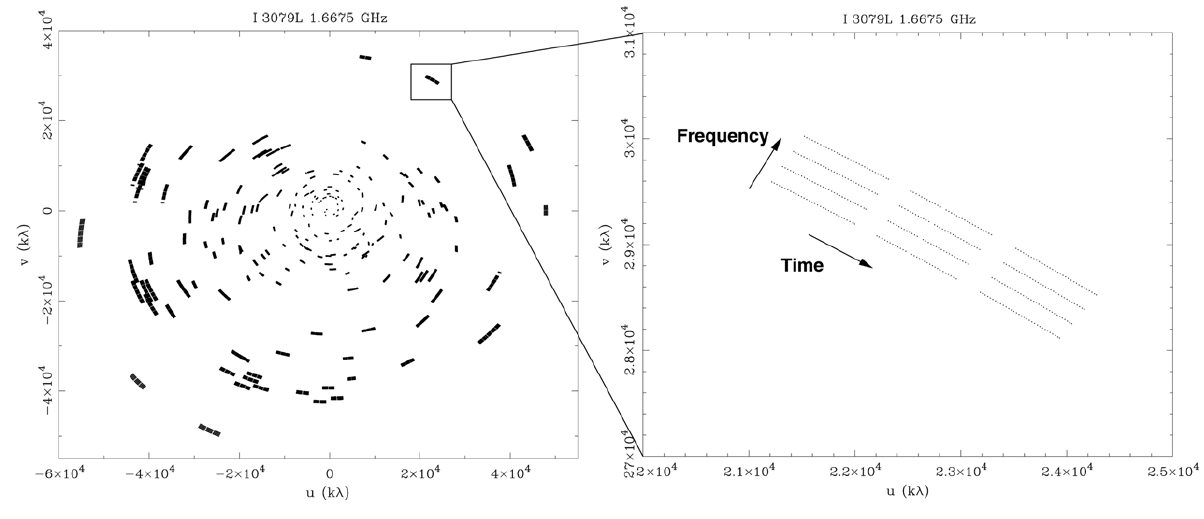
\includegraphics[width=0.9\textwidth]{images/radial_smeering.png}
 \caption[The effects of bandwidth and short-time integration]{The effect of higher frequency components in the bandlimited sampling process manifests itself as orthogonal concentric 
 curves in u,v space, while the effects of short time averaging is smearing in a radial direction. The effect becomes more apparent near the edges of the u,v space \cite{middelberg2008high}.}
  \label{fig_radial_smeering}
 \end{mdframed}
\end{figure}

 The delay tracking center is, itself, not free from error either. These errors are predominantly due to the antenna's suseptability to wind, the effects of heat on 
 the surface of the antenna or errors made by the equipment used to mechanically stear the reflectors. Special instrumentation like tiltmeters can monitor changes in pointing 
 direction and with fast feedback these can be used to track changes in antenna pointing. Other effects such as those of reflector deformation are less well-studied and can significantly
 alter the beam patterns the antennae. Additional problems such as inadequite timing resolution, quantization errors in the calculation and correction of geometrical 
 delays, and synchronization will also result in pointing error.

 Large arrays typically also require phase correction due to other atmospheric effects. At tropospheric levels this includes both dry (stable) and wet effects (largely variable). The problem grows worse with longer baselines and higher
 frequencies, when the curvature, and variations in water-vapor, of the atmosphere has to be taken into consideration. Calibration for these wet effects rely heavily on measurements of atmospheric conditions at the seperate interferometer elements.
 This data is normally stored as additional tables of information and accompany observations.

 Another high altitude atmospheric effect dependent on frequency are the Ionospheric phase delay effects ($\propto \upsilon^{-1}$). The electron column densities are measured by high frequency radar examination (an \textit{ionosonde}) or by dual 
 frequency satellite transmission. These effects additionally vary with direction, as the electron density in the ionosphere is not constant over the entire field of view. The frequency dependency of the ionospheric term is 
 normally calibrated by observing a bright source with a flat spectrum over the observed frequency band. These frequency dependency luckily vary slowly with time and only one such calibration is normally needed per observation.

 Magnetic effects in the Ionosphere typically produces directionally dependent \textit{Faraday Rotation} which introduces a phase rotation between the R and L polarization feeds and additionally
 varies with frequency as well ($\propto \upsilon^{-2}$). Polarization delays are calibrated through strongly polarized sources. Calibration is additionally needed to accomodate for leakage between 
 orthogonal polarizations. Both the troposphere and ionosphere additionally absorbs some of the source signal and contributes to the noise levels in the signal. These can normally be corrected by 
 observing a source of known flux or tipping curve techniques.
 
 Correcting for known time-uniform directional effects can be achieved through either a facet-based polyhedron approach or through AW-projection. Using a image-space facet-based approach these directional
 effects are locally-invariant and are corrected for over small portions of the final image, by multiplying with the appropriate inverse Jones matricies. In AW-projection these effects can be corrected for by convolving with
 transposed Jones matricies, and this can be integrated to either the convolutional gridding (reverse Fast Fourier Transform) or degridding (forward Fast Fourier Transform) strategies which will be discussed 
 in the next chapter \cite{2011A&A...527A.107S}. Both facet-based and AW-projection approaches will be discussed further in the chapter on non-coplanar wide-field imaging.
 
 Another approach is to subtract the directionally dependent effects directly from the observed visibilities, before correcting for the directional independent effects at the model
 subtraction phase. Such an approach corrects these effects individually per model source and is equivalent to evaluating equation~\ref{eqn_RIME} for a set of discrete sources. These
 analytical approaches are computationally prohibative, when compared to the convolution gridding approaches, coupled with either W-projection-based or faceting techniques, although 
 it has the advantage of being much more accurate \cite{2011A&A...527A.107S}.
 
\subsubsection{Self-calibration}
 The lack of strong calibrators near observed areas, and the requirements placed on the properties of these calibrations, makes the process of calibrating the rapidly varying 
 directional effects within the atmosphere a very hard problem. By allowing the individual element gains to be free parameters forms the basis of self-calibration. 

 Self-calibration imposes some restrictions: information about the absolute position, structure and intensity of an observed source is traded
 for improved signal-to-noise ratios. It should be noted that these minimization approaches cannot completely replace the methods of source and polarization calibration mentioned earlier. 
 The effect of these issues are normally incorporated as explicit Jones terms in the model, such as the one mentioned earlier. These effects are greatly reduced by adding additional 
 antennae to the array. The self-calibration problem can be viewed as iteratively improving an initial model by correcting the effects of gain on sky brightness through algorithms such as the Maximum Entropy Method
 and the CLEAN algorithm. The specification of the initial model does not necessarily have to be very accurate for CLEAN to converge at some point: it may simply 
 consist of point sources for relatively simple images. Convergence is, however, not guarenteed.

 The H\"ogbom CLEAN algorithm locates (and keeps a list of) the brightest sources in an image in an iterative cycle, subtracting the Point Spread Function from each source until some 
 thresholding condition is met. The remaining image is termed the residuals. After convolving the found point sources with elliptical function fitted over the Point Spread Function, 
 the residuals are added to the convolved image, forming the final ''clean" image. Many other variations on the algorithm exist, bringing with them improvements in execution speed and 
 stability.

 While CLEAN provides a procedural approach to deconvolution, the Maximum Entropy Method selects an image that fits the data to within a specified noise level, and is not procedural.
 The method essentially limits the range of pixel values and focusses these ranges around bright objects. Though CLEAN is usually much faster on smaller simple images, it is prohibatively slow 
 on large complex images. Under these conditions the Maximum Entropy Method is outright faster.

 Traditional self-calibration, however, assumes that the same ``apparent sky'' is sampled by all antennae, and solves only for the direction independent gain terms. They consider directional dependent terms as simple effects that 
 do not vary in time and is identical per antenna. The addition of directional dependencies within the all-sky integral, primarily those caused by the ionosphere and modulation effects by the primary beam, violates this premis. In 
 the NEWSTAR package the traditional self calibration process includes the following steps \cite{2011A&A...527A.107S}:
 \begin{enumerate}
  \item Gain minimization per antenna, and the minimization of the residual amplitudes and phases associated to each individual baseline (\textit{closure errors}) through a least squares approach.
  \item Model subtraction to form a residual image.
  \item Imaging, deconvolution and model updating using H\"ogbom CLEAN
 \end{enumerate}
 
 In reality this simple least-squares gain-adjustment process cannot remove the effects due to polarized beam patterns, beam rotations and attenuation, as well as the aforementioned effects of the ionosphere and fast-varying tropospheric
 effects. These directionally dependant effects are not simply a multiplication in u,v space, but should be thought of as a convolution. Because these effects vary with both direction and time, deconvolving them is an extremely tricky proposition: 
 at every timestep since only a handful of points from these convolving functions are sampled! More recently several solutions to solve slow-varying Directional Dependent Effects using self-calibration have been proposed. These include pointing self-calibration,
 peeling, the method of differential gains and other compressive sensing techniques (like the analytical solution descibed in \cite{hardy2013direct}). Peeling is a slightly modified version of traditional self-calibration and is widely tested. It involves iteratively removing the effects from the brightest sources, while 
 differential gains simultaniously solves for the gain effects from bright and faint sources using a mix of Direct Fourier Transform and traditional Discrete Fourier Transform-based approaches \cite{2011A&A...527A.107S,2011A&A...527A.108S}.
 
 \section{The imaging and deconvolution cycle}
 There are generally two techniques used to approximate the fourier transforms between the observed visibilities and the (dirty) image. Either a brute force Direct Fourier Transform is taken where each grid point is approximated through a brute-force
 evaluation over all the observed visibilities (M of them in total). This approach requires on the order of $O(N^2M) \approx O(N^4)$ sine and cosine evaluations (where N is the size of a single dimension of a square grid) for a large number of visibilities. A basic co-planar analytical 
 algorithm boils down to a summation of complex multiplications over the entire grid in the image space \cite[Lecture 7]{taylor1999synthesis}: 
 \begin{equation}
  (\forall \text{polarizations})(\forall l,m) I_{p}(l,m) = \frac{1}{M}\sum_{k=1}^{M}{V_p'(u_k,v_k)e^{2\pi i (u_kl,v_km)}}
 \end{equation}
 
 The second approach is to interpolate the data onto a regularly sampled grid with a two-dimensional convolution function, as is required when using the Fast Fourier Transform to approximate the transformations. A Fast Fourier Transform has a computational complexity of $O(N^2\log_2{N})$, while
 convolutional gridding typically requires $O(MC^2) \approx O(N^2C^2)$ operations (where C is the size of each dimension of a square filter) for large numbers of visibilities. If both the image size is small and the number of visibilities 
 are small the Direct Fourier Transform may be faster than the convolutional gridding approach. However, this will not generally be true for very large arrays such as the SKA or its predicessors that are currently under construction, 
 considering the sheer number of baselines involved, as well as the typical grid sizes involved.
 
 An abstract view of imaging, deconvolution and gain correction is shown in figure~\ref{fig_image_cycle}. Experiments performed by Varbanscu et al. \cite{varbanescu2008performance} show that convolutional 
 gridding accounts for nearly 35.4\% of the computation time, while the inverse process of degridding accounts for 48.74\% of a simple gridding and degridding cycle. In this chapter we will primarily focus on the convolutional gridding algorithm, optimal
 convolution functions and a brief overview of the inverse process is given. The next chapter discusses the problem of non-coplanar widefield imaging and the tradeoffs between the various solutions to the 
 problem. Therefore, the w term is, for the moment, not considered in this discussion.
 \begin{figure}[h]
 \begin{mdframed}
 \centering
 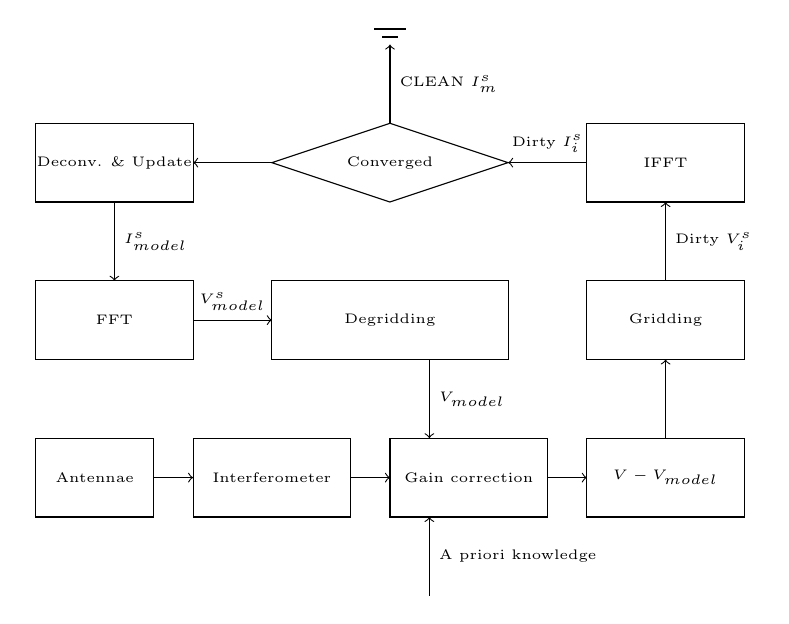
\begin{tikzpicture}[font=\tiny]
    \draw (0,0) rectangle (1.5,1) node at (0.75,0.5) {Antennae};
    \draw[->] (1.5,0.5) -- (2,0.5);
    \draw (2,0) rectangle (4,1) node at (3,0.5) {Interferometer};
    \draw[->] (4,0.5) -- (4.5,0.5);
    \draw (4.5,0) rectangle (6.5,1) node at (5.5,0.5) {Gain correction};
    \draw[->] (6.5,0.5) -- (7,0.5);
    \draw (7,0) rectangle (9,1) node at (8,0.5) {$V - V_{model}$};
    \draw[->] (8,1) -- (8,2);
    \draw (7,2) rectangle (9,3) node at (8,2.5) {Gridding};
    \draw[->] (8,3) -- (8,4) node[pos=.5, right]{Dirty $V_i^s$};
    \draw (7,4) rectangle (9,5) node at (8,4.5) {IFFT};
    \draw[->] (7,4.5) -- (6,4.5) node[pos=.5, above]{Dirty $I_i^s$};
    \draw (3,4.5) -- (4.5,4) -- (6,4.5) -- (4.5,5) -- cycle node at (4.5,4.5) {Converged};
    \draw[->] (3,4.5) -- (2,4.5);
    \draw (0,4) rectangle (2,5) node at (1,4.5) {Deconv. \& Update};
    \draw[->] (1,4) -- (1,3) node[pos=.5, right]{$I_{model}^s$};
    \draw (0,2) rectangle (2,3) node at (1,2.5) {FFT};
    \draw[->] (2,2.5) -- (3,2.5) node[pos=.5, above]{$V_{model}^s$};
    \draw (3,2) rectangle (6,3) node at (4.5,2.5) {Degridding};
    \draw[->] (5,2) -- (5,1) node[pos=.5, right]{$V_{model}$};
    \draw[->] (4.5,5) -- (4.5,6) node[pos=.5, right]{CLEAN $I_m^s$};
    \draw[style=thick] (4.4,6.1) -- (4.6,6.1);
    \draw[style=thick] (4.3,6.2) -- (4.7,6.2);
    \draw[->] (5,-1) -- (5,0) node[pos=.5, right]{A priori knowledge};
 \end{tikzpicture}
 \caption[Imaging pipeline]{The traditional imaging and deconvolution cycle. At the start of the cycle the data is flagged by the observer and known calibration and gain terms are provided.
 An Inverse Fast Fourier Transform is taken after the observed visibilities are uniformly gridded. This dirty sampled image is subsequently deconvolved and the model image updated as per 
 described in the previous section. After this an estimate of the deconvolved visibilities are obtained through an FFT and degridding process, depending on the approach taken. Normally several iterations 
 of this expensive self-calibration cycle is required to converge to a final image of reasonable quality. The directionally dependent effects can be reduced during either gridding 
 or degridding processes for an FFT-based approach. Analytical methods may vary significantly from this illustration.}
 \label{fig_image_cycle}
 \end{mdframed}
 \end{figure}
 
 Exploiting the computational efficiency of the Cooley-Tukey Fast Fourier Transform and its inverse to compute the forward and inverse Discrete Fourier Transforms requires, amongst other considerations, that
 the input is regularly sampled. This sampling is achieved through the process of convolutional gridding. In essense the algorithm can be broken down to four steps as illustrated in figure~\ref{fig_gridding}:
 \begin{enumerate}
  \item The individual complex visibilities are convolved with a highly oversampled function C(u,v). This process spreads them out accross a much wider area in u,v space.
  \item Afterwards the u,v space is regularly sampled.
  \item The image is computed through an Inverse Fast Fourier Transform
  \item A correcting function is applied to the sampled image.
 \end{enumerate}
 \begin{figure}[h]
  \begin{mdframed}
   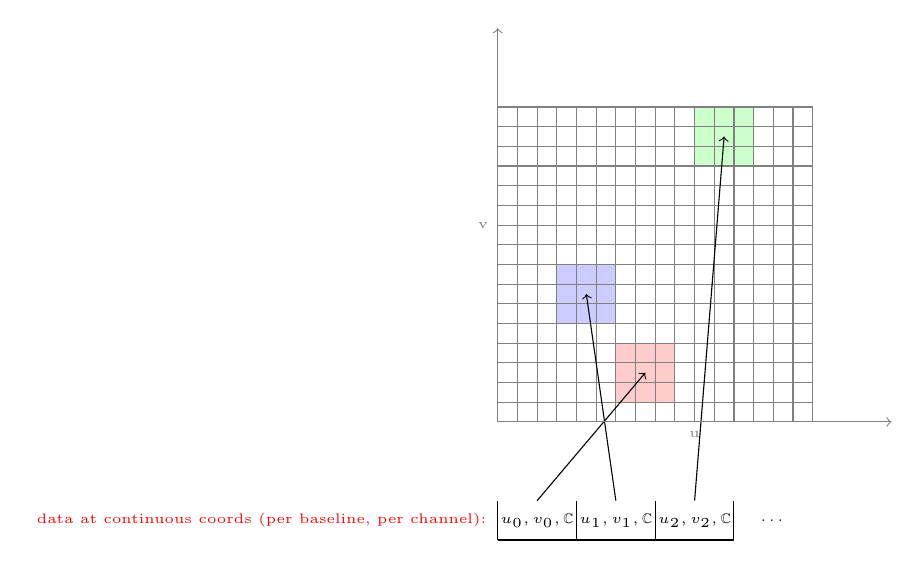
\begin{tikzpicture}[font=\tiny]
    \filldraw[fill=red!20] (4.50,1.75) rectangle (5.25,2.5);
    \filldraw[fill=blue!20] (3.75,2.75) rectangle (4.50,3.50);
    \filldraw[fill=green!20] (5.50,4.75) rectangle (6.25,5.5);
    \draw[step=0.25,gray,thin] (3,1.5) grid (7,5.5);
    \draw[red] node at (0,0.25) {data at continuous coords (per baseline, per channel):};
    \draw node at (6.5,0.25) {\dots};
    \draw[step=1,black] (3,0) grid (6,0.5);
    \draw node at (3.5,0.25) {$u_0,v_0,\mathbb{C}$};
    \draw node at (4.5,0.25) {$u_1,v_1,\mathbb{C}$};
    \draw node at (5.5,0.25) {$u_2,v_2,\mathbb{C}$};
    \draw[->] (3.5,0.5) -- (5-0.125,2.25-0.125);
    \draw[->] (4.5,0.5) -- (4.25-0.125,3.25-0.125);
    \draw[->] (5.5,0.5) -- (6-0.125,5.25-0.125);
    \draw[->,gray] (3,1.5) -- (8,1.5) node[below,pos=0.5]{u};
    \draw[->,gray] (3,1.5) -- (3,6.5) node[left,pos=0.5]{v};
   \end{tikzpicture}
   \caption[Illustration of convolutional gridding]{Each observed visibility (per frequency channel and baseline) is centered at a precomputed coordinate in u,v space and is convolved with 
    some densely sampled function C and binned in a regularly spaced grid. This process essentially spreads each visibility out over a larger area in u,v space. The convolution function is typically sampled
    up to 100 times more regularly than the grid itself \cite{varbanescu2008performance,cornwell2007impact}. It should be clear that this is not the standard convolution as discussed earlier. The fact that the u,v coordinates may vary 
    significantly per baseline may result in two overlapping regions (this poses a problem when parallelizing the algorithm, as will be discussed later on). After all the observed visibilities have been gridded an 
    Inverse Fast Fourier Transform is performed and a correcting function is applied. Each polarization term is typically gridded and transformed to its own, independent, image.}
   \label{fig_gridding}
  \end{mdframed}
 \end{figure}
 Typically the u,v plane is only sparcely sampled as the earth rotates the baselines in u,v space as discussed earlier. This subsampling has the effect of multiplying the observed visibilities with a sampling function. It is also
 not uncommon to find that the u,v space is not uniformly sampled, as pointed out earlier, and that most of the samples are concentrated towards the center of the plane. It is convenient to weigh each sample with its neighbourhood density 
 (the number of visibilities in a neighborhood of grid cells) when sampling sources with both large- and small-scale structure. Natural sampling (typically a weight equal to 1) is used to detect faint sources. After fourier transform
 (by the convolution theorem) the transform of the sampling function is convolved with the image. In image space it is also generally referred to as the Point Spread Function or ``Dirty Beam''. It is possible to remove
 the effects of the Point Spread Function through deconvolution, but deconvolution generally requires a sufficient number of samples to obtain a satisfactory inverse \cite{taylor1999synthesis}.
 
 This sampled observed visibility plane is then convolved with a densely sampled convolution function. The primary goal of this convolution is to interpolate each visibility, but may also limit the aliasing energy outside the support 
 region of the convolving function, as well as limit the interpolation error introduced by using convolutional gridding, instead of the Direct Fourier Transform. Depending on the metrics used to define ``optimal gridding function'' these may vary from a simple truncated sinc or exponential function 
 \cite[Lecture 7]{taylor1999synthesis} to prolate spheriodal functions and approximations to these functions, such as the Keiser Bessel function \cite{jackson1991selection}. Sze Tan \cite{tan1986aperture} derives functions that out-perform prolate spheriodal functions
 on the basis of minimizing aliasing energy, as well as providing an opportunity to trade off the order of interpolation over the area for which the convolution error is small.
 
 It is possible to combine these operations into 
 \begin{equation*}
  I^s_{dirty} = ([I(l,m)*\mathcal{F}^{-1}\{PSF(u,v)\}]\cdot\mathcal{F}^{-1}\{C(u,v)\}) * \mathcal{F}^{-1}\{III(u,v)\}
 \end{equation*}
 \section{The problem of non-coplanar baselines and wide-field imaging}
 Evaluating a direct 3D analytical solution over an image cube with n layers soon becomes intractable for large images, specifically in terms of sheer memory requirements for storing these layers. Over a three dimensional cube, M (the number of visibilities),
 will be reasonably sparcely sampled, and the number of complex multiplications needed per visibility is estimated to be $\frac{4\lambda B_{max}^3}{D^4}$ \cite{yashar2009tdp}. However, the approach remains embarisingly parallel and can
 be scalled over multiple multicore accelerators. A detailed comparison between the throughput achievable by using an analytical approach, compared to convolutional gridding approaches have not been for multicore accelerators \cite{hardy2013direct}.

%  \section{Review of core signals processing techniques}
% Radio astronomy has its roots in Digital Signals Processing. Before diving into the details of how these telescopes work we refer the reader to the \textit{Scientist and Engineer's guide to Digital Signals Processing} by 
% Steven Smith\footnote{Available freely at \url{http://www.dspguide.com/}}\cite{smith1997scientist} for a detailed, yet simple overview of the field. A (very) brief overview of some of the core terminology is given here.
% 
% A signal is simply a description of how one parameter depends on another. A typical example of this is how voltage varies over time. Since the focus in this thesis lie solely in digitized signals, it is necessary to carefully
% define under what circumstances the underlying continuous analog signal can be reconstructed. The Shannon-Nyquest \textit{sampling theorem} forms the cornerstone of Digital Signals Processing. It simply states that the rate at
% which samples are taken from a continuous signal has to be at least twice the highest frequency component of that signal. Such a signal is said to be critically sampled if it obeys this minimum requirement. If the requirement is
% not satisfied the sampled signal is aliased (higher frequencies appear as low frequency com on gradebook and assignments tab yesterday on vula, so I thought I should contact you to know whether this is known to you. I don't know what happened but I had marks before. Thank you!ponents). This can be illustrated through figure~\ref{fig_invalid_sampling}. Aliasing is usually reduced by applying a filter that essentially
% have low responses at frequencies outside a limited \text{passband} of frequencies. This filter is can be something as simple as a windowed sinc function for instance. Although a sharp cutoff frequency is ideal, it should be noted 
% that in reality this is not achieved. Filter frequency responces usually decline over a non-infinitesimal section of the spectrum (this is known as \textit{rolloff}).
% 
% \begin{figure}[ht]
%  \begin{mdframed}
%  \centering
%  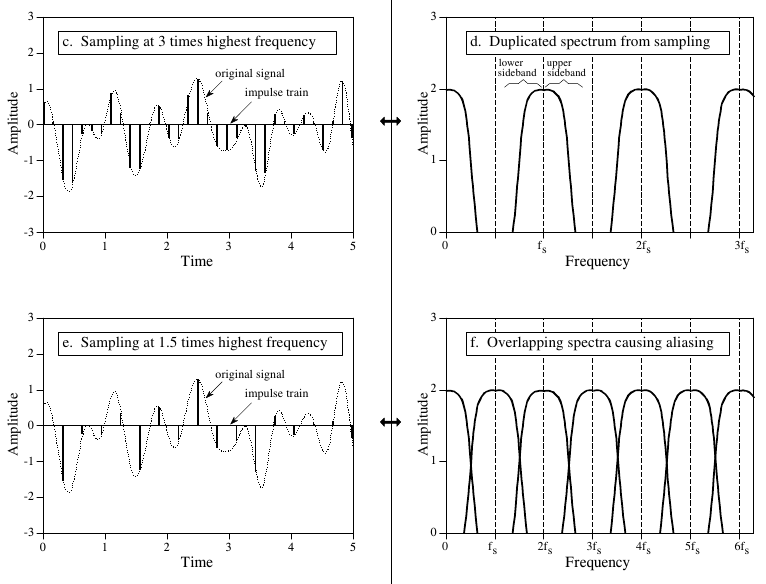
\includegraphics[width=0.8\textwidth]{images/improper_sampling.png}
%  \caption[Aliasing]{The first signal is sampled at 3 times the highest composing frequency. Its frequency spectrum shows no overlap between sidebands. The second signal is subsampled and higher frequencies overlap lower frequencies
%  in its frequency spectrum. This illustrates a key observation: discarding samples in one domain causes aliasing in the other \cite{smith1997scientist}.}
%  \label{fig_invalid_sampling}
%  \end{mdframed}
% \end{figure}
% 
% The next observation is that the propogation of electromagnetic waves and their interactions can be considered as a linear system. This means the signals exhibit three properties: homogeneity, additivity and shift-invariance (the third 
% is a non-compulsory property of linearity). We say that the following are true for such systems:
% 
%   \begin{flalign*}
%     &\textbf{ if }x[n] \rightarrow \text{System} \rightarrow y[n] \textbf{ then } k x[n] \rightarrow \text{System} \rightarrow k y[n] \textit{ (homogeneity)}\\
%     &\textbf{ if }x_1[n] \rightarrow \text{System} \rightarrow y_1[n]\textbf{ and }x_2[n] \rightarrow \text{System} \rightarrow y_2[n] \textbf{ then } x_1[n] + x_2[n] \rightarrow \text{System} \rightarrow y_1[n] + y_2[n] \textit{ (additivity)}\\
%     &\textbf{ if }x[n] \rightarrow \text{System} \rightarrow y[n] \textbf{ then } x[n + s] \rightarrow \text{System} \rightarrow y[n + s] \textit{ (shift-invariance)}&
%   \end{flalign*}
% 
% Much of the filtering and imaging techniques described in this thesis rely on the theory of fourier transforms. The fourier transform simply decomposes a continuous periodic signal into a series of sinusoidal terms. A detailed description 
% can be found in Smith \cite[ch 8-12,31]{smith1997scientist}, but the general relations between converting between the time and frequency domains (and between the visibility and the intensity spaces as will be described later on) are as follows:
% \begin{equation*}
%   \begin{split}
%     G(f) &= \int_{-\infty}^{\infty}g(x)e^{2\pi ifx}\\
%     g(x) &= \int_{-\infty}^{\infty}G(f)e^{-2\pi ifx}
%   \end{split}
% \end{equation*}
% Here capital letters indicate the Fourier space. We will be using this convention throughout this thesis. It is also possible to do this with discrete signals (indicated with square brackets as per convention). In that case the Cooley-Tukey Fast 
% Fourier Transform algorithm and its inverse is employed to move between these domains. There are highly optimized libraries available for both C++ (FFTW) and CUDA (cuFFT), and these will be extensively used in our implementations.
% 
% For linear systems the following theorems are true (stated without proof):
% \begin{equation*}
%   \begin{split}
%     g_1(x)*g_2(x) &:= \int_{-\infty}^{\infty}g_1(t)g_2(x-t)\textit{ (convolution)}\\
%     g_1(x)\star g_2(x) &:= \int_{-\infty}^{\infty}g_1(t)g_2(t+x)\textit{ (cross-correlation)}\\
%     &=g_1^*(-x)*g_2(x)\\
%     \text{Addition Theorem:}\\
%     \mathcal{F}(g_1(x)+g_2(x)) &= G_1(f)+G_2(f)\\
%     \text{Convolution Theorem:}\\
%     \mathcal{F}(g_1(x)*g_2(x)) &=G_1(f).G_2(f)\\
%     \mathcal{F}(g_1(x).g_2(x)) &=G_1(f)*G_2(f)\\
%     \text{Shift Theorem:}\\
%     \mathcal{F}(g(x-\Delta))&=G(f)e^{-2\pi if\Delta}
%   \end{split}
% \end{equation*}
% 
% In general the convolution is known as filtering, the cross-correlation can be seen as ``time averaging between two signals'' and signal shifting essentially shifts the directional cosine (as seen in the next section) and electrically
% stears the telescope. The two dimensional versions of convolution, cross-correlation, the fourier transform and its inverse are analoguous to their one dimensional counterparts. The two dimensional fourier transform first transforms
% over one axis and then transforms the output on the second axis.
 
\bibliography{bibfile}
\bibliographystyle{plain}
\end{document}          
